\section{寄存器描述}
\regover{
{\hyperref[i2c-i2c-config]{i2c\_config}}&Master configure
\\
\hline
{\hyperref[i2c-i2c-int-sts]{i2c\_int\_sts}}&Interrupt configure and status
\\
\hline
{\hyperref[i2c-i2c-sub-addr]{i2c\_sub\_addr}}&Sub-address setting
\\
\hline
{\hyperref[i2c-i2c-bus-busy]{i2c\_bus\_busy}}&Bus busy status
\\
\hline
{\hyperref[i2c-i2c-prd-start]{i2c\_prd\_start}}&Start period setting
\\
\hline
{\hyperref[i2c-i2c-prd-stop]{i2c\_prd\_stop}}&Stop period setting
\\
\hline
{\hyperref[i2c-i2c-prd-data]{i2c\_prd\_data}}&Data period setting
\\
\hline
{\hyperref[i2c-i2c-fifo-config-0]{i2c\_fifo\_config\_0}}&FIFO status and DMA mode
\\
\hline
{\hyperref[i2c-i2c-fifo-config-1]{i2c\_fifo\_config\_1}}&FIFO threshold and available count
\\
\hline
{\hyperref[i2c-i2c-fifo-wdata]{i2c\_fifo\_wdata}}&TX FIFO
\\
\hline
{\hyperref[i2c-i2c-fifo-rdata]{i2c\_fifo\_rdata}}&RX FIFO
\\
\hline
}

\subsection{i2c\_config}
\label{i2c-i2c-config}
地址:0x40018000
 \begin{figure}[H]
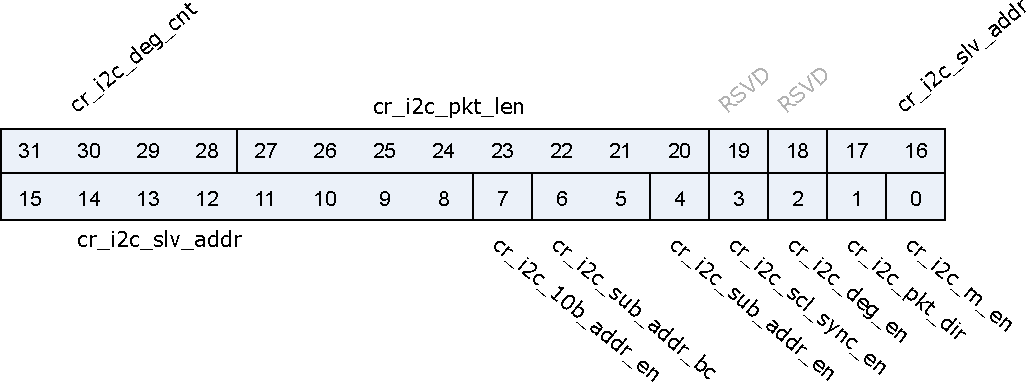
\includegraphics{i2c_i2c_config.pdf}
\end{figure}

\regdes{31:28&cr\_i2c\_deg\_cnt&r/w&4'd0&De-glitch function cycle count\\\hline
27:20&cr\_i2c\_pkt\_len&r/w&8'd0&Packet length (unit: byte)\\\hline
19:18&RSVD& & & \\\hline
17:8&cr\_i2c\_slv\_addr&r/w&10'h0&Slave address for I2C transaction (target address)\\\hline
7&cr\_i2c\_10b\_addr\_en&r/w&1'b0&Slave address 10-bit mode enable\\\hline
6:5&cr\_i2c\_sub\_addr\_bc&r/w&2'd0&Sub-address field byte count \par 2'd0: 1-byte, 2'd1: 2-byte, 2'd2: 3-byte, 2'd3: 4-byte
\\\hline
4&cr\_i2c\_sub\_addr\_en&r/w&1'b0&Enable signal of I2C sub-address field\\\hline
3&cr\_i2c\_scl\_sync\_en&r/w&1'b1&Enable signal of I2C SCL synchronization, should be enabled to support Multi-Master and Clock-Stretching \par (Normally should not be turned-off)
\\\hline
2&cr\_i2c\_deg\_en&r/w&1'b0&Enable signal of I2C input de-glitch function (for all input pins)\\\hline
1&cr\_i2c\_pkt\_dir&r/w&1'b1&Transfer direction of the packet \par 1'b0: Write; 1'b1: Read
\\\hline
0&cr\_i2c\_m\_en&r/w&1'b0&Enable signal of I2C Master function \par Asserting this bit will trigger the transaction, and should be de-asserted after finish
\\\hline

}
\subsection{i2c\_int\_sts}
\label{i2c-i2c-int-sts}
地址:0x40018004
 \begin{figure}[H]
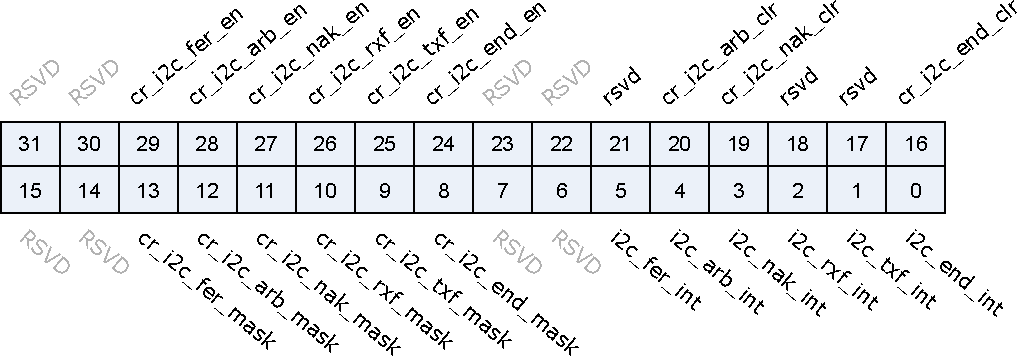
\includegraphics{i2c_i2c_int_sts.pdf}
\end{figure}

\regdes{31:30&RSVD& & & \\\hline
29&cr\_i2c\_fer\_en&r/w&1'b1&Interrupt enable of i2c\_fer\_int\\\hline
28&cr\_i2c\_arb\_en&r/w&1'b1&Interrupt enable of i2c\_arb\_int\\\hline
27&cr\_i2c\_nak\_en&r/w&1'b1&Interrupt enable of i2c\_nak\_int\\\hline
26&cr\_i2c\_rxf\_en&r/w&1'b1&Interrupt enable of i2c\_rxf\_int\\\hline
25&cr\_i2c\_txf\_en&r/w&1'b1&Interrupt enable of i2c\_txf\_int\\\hline
24&cr\_i2c\_end\_en&r/w&1'b1&Interrupt enable of i2c\_end\_int\\\hline
23:22&RSVD& & & \\\hline
21&rsvd&rsvd&1'b0&\\\hline
20&cr\_i2c\_arb\_clr&w1c&1'b0&Interrupt clear of i2c\_arb\_int\\\hline
19&cr\_i2c\_nak\_clr&w1c&1'b0&Interrupt clear of i2c\_nak\_int\\\hline
18&rsvd&rsvd&1'b0&\\\hline
17&rsvd&rsvd&1'b0&\\\hline
16&cr\_i2c\_end\_clr&w1c&1'b0&Interrupt clear of i2c\_end\_int\\\hline
15:14&RSVD& & & \\\hline
13&cr\_i2c\_fer\_mask&r/w&1'b1&Interrupt mask of i2c\_fer\_int\\\hline
12&cr\_i2c\_arb\_mask&r/w&1'b1&Interrupt mask of i2c\_arb\_int\\\hline
11&cr\_i2c\_nak\_mask&r/w&1'b1&Interrupt mask of i2c\_nak\_int\\\hline
10&cr\_i2c\_rxf\_mask&r/w&1'b1&Interrupt mask of i2c\_rxf\_int\\\hline
9&cr\_i2c\_txf\_mask&r/w&1'b1&Interrupt mask of i2c\_txf\_int\\\hline
8&cr\_i2c\_end\_mask&r/w&1'b1&Interrupt mask of i2c\_end\_int\\\hline
7:6&RSVD& & & \\\hline
5&i2c\_fer\_int&r&1'b0&I2C TX/RX FIFO error interrupt, auto-cleared when FIFO overflow/underflow error flag is cleared\\\hline
4&i2c\_arb\_int&r&1'b0&I2C arbitration lost interrupt\\\hline
3&i2c\_nak\_int&r&1'b0&I2C NACK-received interrupt\\\hline
2&i2c\_rxf\_int&r&1'b0&I2C RX FIFO ready (rx\_fifo\_cnt > rx\_fifo\_th) interrupt, auto-cleared when data is popped\\\hline
1&i2c\_txf\_int&r&1'b1&I2C TX FIFO ready (tx\_fifo\_cnt > tx\_fifo\_th) interrupt, auto-cleared when data is pushed\\\hline
0&i2c\_end\_int&r&1'b0&I2C transfer end interrupt\\\hline

}
\subsection{i2c\_sub\_addr}
\label{i2c-i2c-sub-addr}
地址:0x40018008
 \begin{figure}[H]
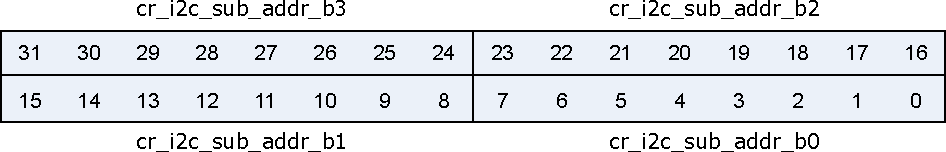
\includegraphics{i2c_i2c_sub_addr.pdf}
\end{figure}

\regdes{31:24&cr\_i2c\_sub\_addr\_b3&r/w&8'd0&I2C sub-address field - byte[3]\\\hline
23:16&cr\_i2c\_sub\_addr\_b2&r/w&8'd0&I2C sub-address field - byte[2]\\\hline
15:8&cr\_i2c\_sub\_addr\_b1&r/w&8'd0&I2C sub-address field - byte[1]\\\hline
7:0&cr\_i2c\_sub\_addr\_b0&r/w&8'd0&I2C sub-address field - byte[0] (sub-address starts from this byte)\\\hline

}
\subsection{i2c\_bus\_busy}
\label{i2c-i2c-bus-busy}
地址:0x4001800c
 \begin{figure}[H]
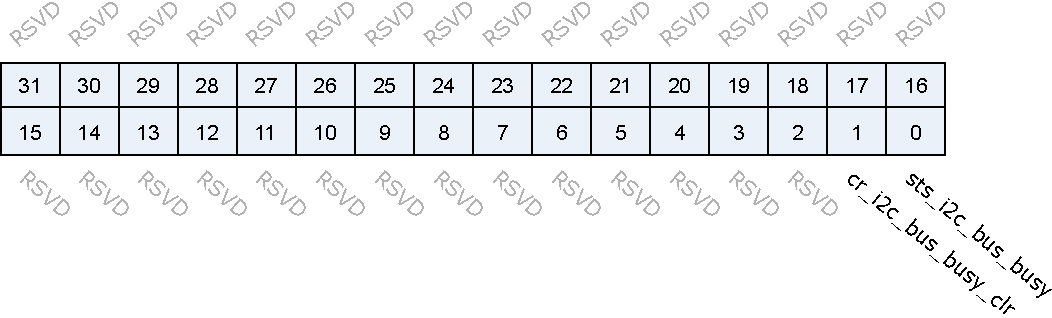
\includegraphics{i2c_i2c_bus_busy.pdf}
\end{figure}

\regdes{31:2&RSVD& & & \\\hline
1&cr\_i2c\_bus\_busy\_clr&w1c&1'b0&Clear signal of bus\_busy status, not for normal usage (in case I2C bus hangs)\\\hline
0&sts\_i2c\_bus\_busy&r&1'b0&Indicator of I2C bus busy \par 0: Idle \par 1: Busy
\\\hline

}
\subsection{i2c\_prd\_start}
\label{i2c-i2c-prd-start}
地址:0x40018010
 \begin{figure}[H]
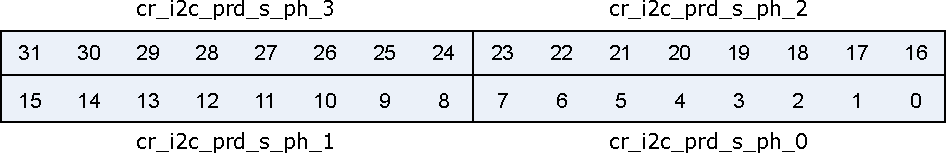
\includegraphics{i2c_i2c_prd_start.pdf}
\end{figure}

\regdes{31:24&cr\_i2c\_prd\_s\_ph\_3&r/w&8'd15&Length of START condition phase 3 (unit: I2C source clock period)\\\hline
23:16&cr\_i2c\_prd\_s\_ph\_2&r/w&8'd15&Length of START condition phase 2 (unit: I2C source clock period)\\\hline
15:8&cr\_i2c\_prd\_s\_ph\_1&r/w&8'd15&Length of START condition phase 1 (unit: I2C source clock period)\\\hline
7:0&cr\_i2c\_prd\_s\_ph\_0&r/w&8'd15&Length of START condition phase 0 (unit: I2C source clock period)\\\hline

}
\subsection{i2c\_prd\_stop}
\label{i2c-i2c-prd-stop}
地址:0x40018014
 \begin{figure}[H]
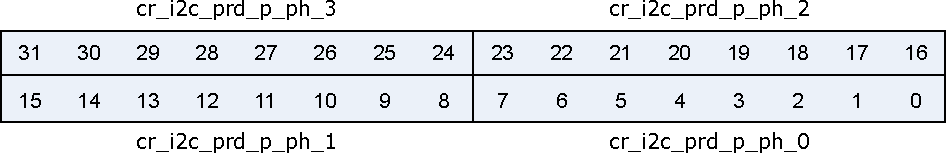
\includegraphics{i2c_i2c_prd_stop.pdf}
\end{figure}

\regdes{31:24&cr\_i2c\_prd\_p\_ph\_3&r/w&8'd15&Length of STOP condition phase 3 (unit: I2C source clock period)\\\hline
23:16&cr\_i2c\_prd\_p\_ph\_2&r/w&8'd15&Length of STOP condition phase 2 (unit: I2C source clock period)\\\hline
15:8&cr\_i2c\_prd\_p\_ph\_1&r/w&8'd15&Length of STOP condition phase 1 (unit: I2C source clock period)\\\hline
7:0&cr\_i2c\_prd\_p\_ph\_0&r/w&8'd15&Length of STOP condition phase 0 (unit: I2C source clock period)\\\hline

}
\subsection{i2c\_prd\_data}
\label{i2c-i2c-prd-data}
地址:0x40018018
 \begin{figure}[H]
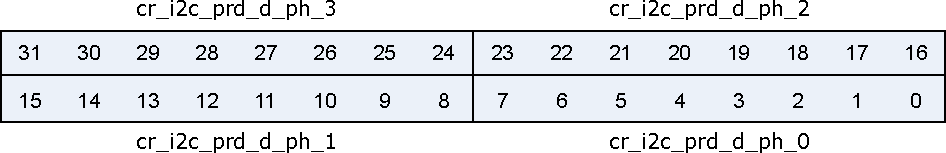
\includegraphics{i2c_i2c_prd_data.pdf}
\end{figure}

\regdes{31:24&cr\_i2c\_prd\_d\_ph\_3&r/w&8'd15&Length of DATA phase 3 (unit: I2C source clock period)\\\hline
23:16&cr\_i2c\_prd\_d\_ph\_2&r/w&8'd15&Length of DATA phase 2 (unit: I2C source clock period)\\\hline
15:8&cr\_i2c\_prd\_d\_ph\_1&r/w&8'd15&Length of DATA phase 1 (unit: I2C source clock period) \par Note: This value should not be set to 8'd0, adjust source clock rate instead if higher I2C clock rate is required
\\\hline
7:0&cr\_i2c\_prd\_d\_ph\_0&r/w&8'd15&Length of DATA phase 0 (unit: I2C source clock period)\\\hline

}
\subsection{i2c\_fifo\_config\_0}
\label{i2c-i2c-fifo-config-0}
地址:0x40018080
 \begin{figure}[H]
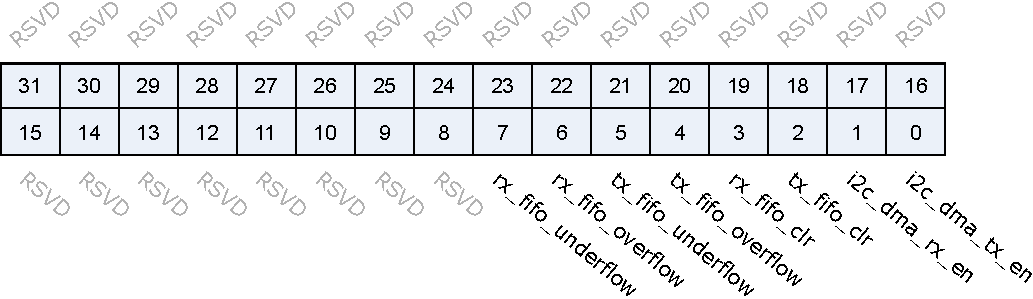
\includegraphics{i2c_i2c_fifo_config_0.pdf}
\end{figure}

\regdes{31:8&RSVD& & & \\\hline
7&rx\_fifo\_underflow&r&1'b0&Underflow flag of RX FIFO, can be cleared by rx\_fifo\_clr\\\hline
6&rx\_fifo\_overflow&r&1'b0&Overflow flag of RX FIFO, can be cleared by rx\_fifo\_clr\\\hline
5&tx\_fifo\_underflow&r&1'b0&Underflow flag of TX FIFO, can be cleared by tx\_fifo\_clr\\\hline
4&tx\_fifo\_overflow&r&1'b0&Overflow flag of TX FIFO, can be cleared by tx\_fifo\_clr\\\hline
3&rx\_fifo\_clr&w1c&1'b0&Clear signal of RX FIFO, RX FIFO will be empty when write 1 to this bit\\\hline
2&tx\_fifo\_clr&w1c&1'b0&Clear signal of TX FIFO, TX FIFO will be empty when write 1 to this bit\\\hline
1&i2c\_dma\_rx\_en&r/w&1'b0&Enable signal of dma\_rx\_req/ack interface\\\hline
0&i2c\_dma\_tx\_en&r/w&1'b0&Enable signal of dma\_tx\_req/ack interface\\\hline

}
\subsection{i2c\_fifo\_config\_1}
\label{i2c-i2c-fifo-config-1}
地址:0x40018084
 \begin{figure}[H]
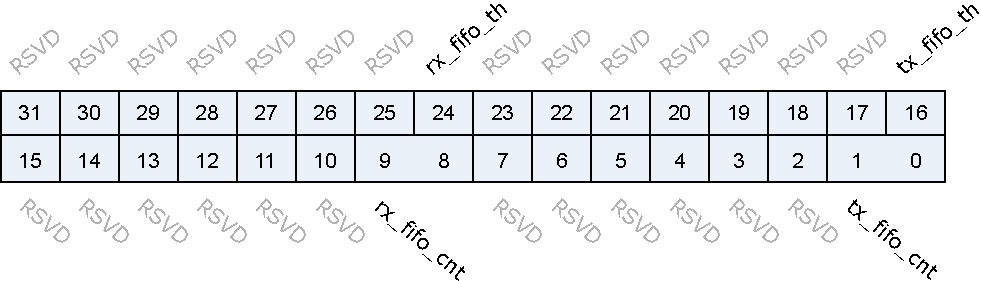
\includegraphics{i2c_i2c_fifo_config_1.pdf}
\end{figure}

\regdes{31:25&RSVD& & & \\\hline
24&rx\_fifo\_th&r/w&1'd0&RX FIFO threshold, dma\_rx\_req will not be asserted if rx\_fifo\_cnt is less than this value\\\hline
23:17&RSVD& & & \\\hline
16&tx\_fifo\_th&r/w&1'd0&TX FIFO threshold, dma\_tx\_req will not be asserted if tx\_fifo\_cnt is less than this value\\\hline
15:10&RSVD& & & \\\hline
9:8&rx\_fifo\_cnt&r&2'd0&RX FIFO available count, means count of data received in RX FIFO\\\hline
7:2&RSVD& & & \\\hline
1:0&tx\_fifo\_cnt&r&2'd2&TX FIFO available count, means empty space remained in TX FIFO\\\hline

}
\subsection{i2c\_fifo\_wdata}
\label{i2c-i2c-fifo-wdata}
地址:0x40018088
 \begin{figure}[H]
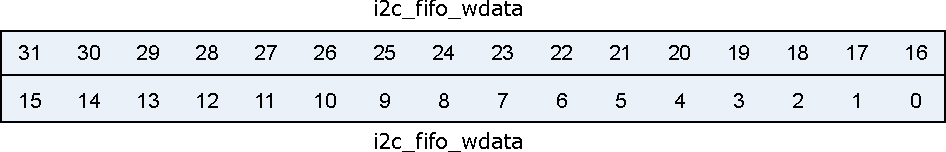
\includegraphics{i2c_i2c_fifo_wdata.pdf}
\end{figure}

\regdes{31:0&i2c\_fifo\_wdata&w&x&TX FIFO, size is 4*2 = 8-byte\\\hline

}
\subsection{i2c\_fifo\_rdata}
\label{i2c-i2c-fifo-rdata}
地址:0x4001808c
 \begin{figure}[H]
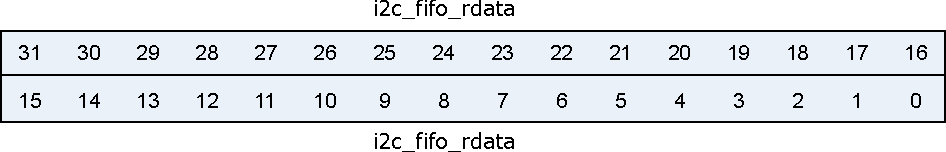
\includegraphics{i2c_i2c_fifo_rdata.pdf}
\end{figure}

\regdes{31:0&i2c\_fifo\_rdata&r&32'h0&RX FIFO, size is 4*2 = 8-byte\\\hline

}
